\documentclass[xcolor=dvipsnames,slidestop,compress,mathserif, 11pt]{beamer}
\usecolortheme[named=Blue]{structure}
\usetheme[height=2mm]{Rochester}
\setbeamerfont{structure}{shape=\itshape}
\mode<presentation> {
\usetheme{Darmstadt} % Tema seleccionado.
\usecolortheme{default}%{albatross} % Color del tema.
\setbeamercovered{transparent} % Transparencia.
}
%\setbeamercovered{transparent}
%}%%%% packages y comandos personales %%%%
\setbeamertemplate{caption}[numbered]
\usepackage{ragged2e}
\usepackage{comment}
\renewcommand{\figurename}{Figura}
\renewcommand{\tablename}{Tabla}
%\usepackage{latexsym} % S��mbolos
\usepackage{amsmath}
\usepackage{array}
\usepackage{amssymb}
\usepackage{wasysym}
\usepackage{stmaryrd}
\usepackage{wrapfig}
\usepackage{multicol}
\usepackage{dsfont,float}
\usepackage{soul}
\usepackage{upgreek}
\usepackage{accents}
\usepackage{physics}
%\usepackage[lite]{mtpro2}
\usepackage{tikz}
\usepackage{lipsum}
\newcommand\Fontvi{\fontsize{6}{7.2}\selectfont}
%\usepackage{turnstile}
\font\shi=cmssdc10 scaled 700
\title[Tesis profesional]{Evoluci\'on de una funci\'on de Wigner de un amplificador param\'etrico}
\author{TESIS PROFESIONAL\\
Carlos Eduardo González Anguiano}
\institute{Departamento de Física ESFM-IPN}
\date{1 de junio de 2024}
\usepackage{graphicx}
%\graphicspath{%
%
%    {E:/Efi1-ggg/}% inserted by PCTeX
%    {/}% inserted by PCTeX
%}
\usepackage[utf8]{inputenc} % Usar latin1 causa error para acentos
\begin{document}


\maketitle


\begin{frame}
	\frametitle{Índice}
	\tableofcontents[pausesections]
\end{frame}

\section{Introducción}

\begin{frame}[c]
	\frametitle{Introducción: Mecánica Cuántica (MC)}
	\textbf{Max Planck y la \textit{catástrofe ultravioleta}}\\
	\justifying \textit{Densidad espectral de energía}: Energía por unidad de volumen de ondas electromagnéticas de frecuencia $\nu$.
	\begin{equation}
		u(T)=\int_{0}^{\infty}\rho(\nu, T)d\nu.
	\end{equation}
	\justifying La densidad de \textit{cuerpo negro} dado por termodinámica clásica difiere de datos experimentales.
	Planck propone estados de energía de osciladores discretos
	\begin{equation}
		E_n = nh\nu.
	\end{equation}
	\justifying La cuantización lleva a la \textit{distribución de Planck}
	\begin{equation}
		\rho(\nu, T) = \frac{\hbar \nu^3}{\pi^2 c^3} \frac{1}{e^{\hbar\nu/kT}-1}.
	\end{equation}
\end{frame}

\begin{frame}
	\begin{figure}[h]
		\centering
		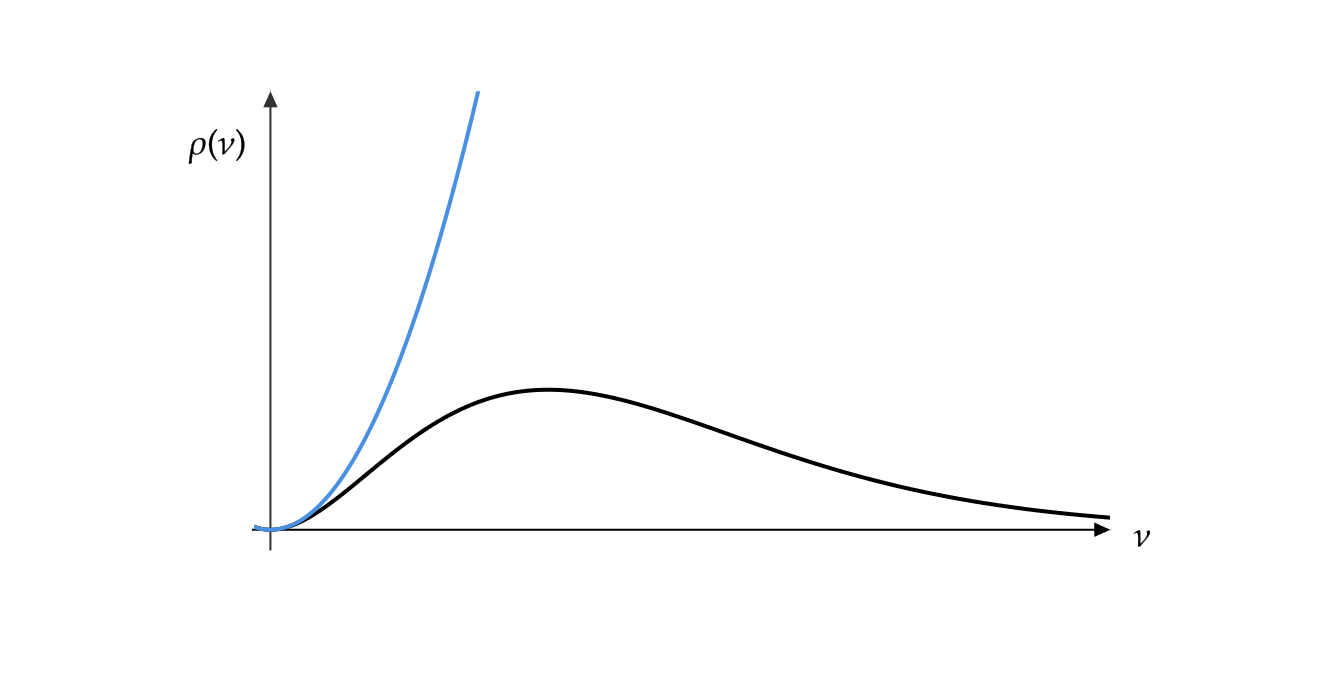
\includegraphics[width=0.75\textwidth]{images/planck-distribution.png}
		\caption{Distribución de Planck (negro) y distribución de Rayleigh-Jeans (azul)}
		\label{fig:dist-planck}
	\end{figure}
\end{frame}

\begin{frame}
	\textbf{Einstein y el \textit{efecto fotoeléctrico}}\\
	\justifying Describe el efecto de la luz incidente sobre un metal, y como este emite electrones.
	\begin{itemize}
		\item La energía máxima de los electrones es independiente a la intensidad.
		\item La energía depende de la frecuencia de la luz incidente
		\item El número de fotones depende de la intensidad
		\item Cada material tiene una frecuencia característica para liberar electrones.
	\end{itemize}
	\justifying Sugiere que la luz puede estar dados por paquetes de energía, llamados después \textit{fotones}. Con ello resuelve dificultades teóricas del experimento. La energía tiene que ser mayor que la función de trabajo $W$ para liberarlo, es decir $\hbar \nu \geq W$.
	\begin{equation}
		\frac{1}{2}mv^2 = \hbar \nu - W
	\end{equation}
\end{frame}

\begin{frame}
	\justifying
	\begin{figure}[h]
		\centering
		\tikzset{every picture/.style={line width=0.75pt}} %set default line width to 0.75pt        
		\resizebox{0.9\columnwidth}{!}{%




			\tikzset{every picture/.style={line width=0.75pt}} %set default line width to 0.75pt        

		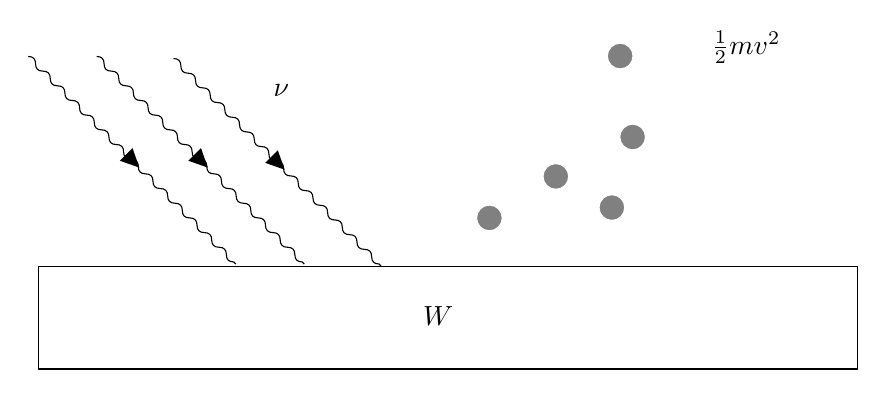
\begin{tikzpicture}[x=0.75pt,y=0.75pt,yscale=-1,xscale=1]
			%uncomment if require: \path (0,474); %set diagram left start at 0, and has height of 474

			%Shape: Rectangle [id:dp23981286336519314] 
			\draw   (124,299) -- (518.6,299) -- (518.6,348.6) -- (124,348.6) -- cycle ;
			%Straight Lines [id:da7445672959470432] 
			\draw    (152,198) .. controls (154.36,198) and (155.54,199.18) .. (155.54,201.54) .. controls (155.54,203.89) and (156.72,205.07) .. (159.07,205.07) .. controls (161.43,205.07) and (162.61,206.25) .. (162.61,208.61) .. controls (162.61,210.96) and (163.79,212.14) .. (166.14,212.14) .. controls (168.5,212.14) and (169.68,213.32) .. (169.68,215.68) .. controls (169.68,218.03) and (170.86,219.21) .. (173.21,219.21) .. controls (175.57,219.21) and (176.75,220.39) .. (176.75,222.75) .. controls (176.75,225.1) and (177.93,226.28) .. (180.28,226.28) .. controls (182.64,226.28) and (183.82,227.46) .. (183.82,229.82) .. controls (183.82,232.18) and (185,233.36) .. (187.36,233.36) .. controls (189.71,233.36) and (190.89,234.54) .. (190.89,236.89) .. controls (190.89,239.25) and (192.07,240.43) .. (194.43,240.43) .. controls (196.78,240.43) and (197.96,241.61) .. (197.96,243.96) .. controls (197.96,246.32) and (199.14,247.5) .. (201.5,247.5) .. controls (203.85,247.5) and (205.03,248.68) .. (205.03,251.03) .. controls (205.03,253.39) and (206.21,254.57) .. (208.57,254.57) .. controls (210.92,254.57) and (212.1,255.75) .. (212.1,258.1) .. controls (212.1,260.46) and (213.28,261.64) .. (215.64,261.64) .. controls (218,261.64) and (219.18,262.82) .. (219.18,265.18) .. controls (219.18,267.53) and (220.36,268.71) .. (222.71,268.71) .. controls (225.07,268.71) and (226.25,269.89) .. (226.25,272.25) .. controls (226.25,274.6) and (227.43,275.78) .. (229.78,275.78) .. controls (232.14,275.78) and (233.32,276.96) .. (233.32,279.32) .. controls (233.32,281.67) and (234.5,282.85) .. (236.85,282.85) .. controls (239.21,282.85) and (240.39,284.03) .. (240.39,286.39) .. controls (240.39,288.74) and (241.57,289.92) .. (243.92,289.92) .. controls (246.28,289.92) and (247.46,291.1) .. (247.46,293.46) .. controls (247.46,295.81) and (248.64,296.99) .. (250.99,296.99) -- (252,298) -- (252,298) ;
			\draw [shift={(205.54,251.54)}, rotate = 225] [fill={rgb, 255:red, 0; green, 0; blue, 0 }  ][line width=0.08]  [draw opacity=0] (8.93,-4.29) -- (0,0) -- (8.93,4.29) -- cycle    ;
			%Straight Lines [id:da889583638371712] 
			\draw    (119,198) .. controls (121.36,198) and (122.54,199.18) .. (122.54,201.54) .. controls (122.54,203.89) and (123.72,205.07) .. (126.07,205.07) .. controls (128.43,205.07) and (129.61,206.25) .. (129.61,208.61) .. controls (129.61,210.96) and (130.79,212.14) .. (133.14,212.14) .. controls (135.5,212.14) and (136.68,213.32) .. (136.68,215.68) .. controls (136.68,218.03) and (137.86,219.21) .. (140.21,219.21) .. controls (142.57,219.21) and (143.75,220.39) .. (143.75,222.75) .. controls (143.75,225.1) and (144.93,226.28) .. (147.28,226.28) .. controls (149.64,226.28) and (150.82,227.46) .. (150.82,229.82) .. controls (150.82,232.18) and (152,233.36) .. (154.36,233.36) .. controls (156.71,233.36) and (157.89,234.54) .. (157.89,236.89) .. controls (157.89,239.25) and (159.07,240.43) .. (161.43,240.43) .. controls (163.78,240.43) and (164.96,241.61) .. (164.96,243.96) .. controls (164.96,246.32) and (166.14,247.5) .. (168.5,247.5) .. controls (170.85,247.5) and (172.03,248.68) .. (172.03,251.03) .. controls (172.03,253.39) and (173.21,254.57) .. (175.57,254.57) .. controls (177.92,254.57) and (179.1,255.75) .. (179.1,258.1) .. controls (179.1,260.46) and (180.28,261.64) .. (182.64,261.64) .. controls (185,261.64) and (186.18,262.82) .. (186.18,265.18) .. controls (186.18,267.53) and (187.36,268.71) .. (189.71,268.71) .. controls (192.07,268.71) and (193.25,269.89) .. (193.25,272.25) .. controls (193.25,274.6) and (194.43,275.78) .. (196.78,275.78) .. controls (199.14,275.78) and (200.32,276.96) .. (200.32,279.32) .. controls (200.32,281.67) and (201.5,282.85) .. (203.85,282.85) .. controls (206.21,282.85) and (207.39,284.03) .. (207.39,286.39) .. controls (207.39,288.74) and (208.57,289.92) .. (210.92,289.92) .. controls (213.28,289.92) and (214.46,291.1) .. (214.46,293.46) .. controls (214.46,295.81) and (215.64,296.99) .. (217.99,296.99) -- (219,298) -- (219,298) ;
			\draw [shift={(172.54,251.54)}, rotate = 225] [fill={rgb, 255:red, 0; green, 0; blue, 0 }  ][line width=0.08]  [draw opacity=0] (8.93,-4.29) -- (0,0) -- (8.93,4.29) -- cycle    ;
			%Straight Lines [id:da20064433994992514] 
			\draw    (189,199) .. controls (191.36,199) and (192.54,200.18) .. (192.54,202.54) .. controls (192.54,204.89) and (193.72,206.07) .. (196.07,206.07) .. controls (198.43,206.07) and (199.61,207.25) .. (199.61,209.61) .. controls (199.61,211.96) and (200.79,213.14) .. (203.14,213.14) .. controls (205.5,213.14) and (206.68,214.32) .. (206.68,216.68) .. controls (206.68,219.03) and (207.86,220.21) .. (210.21,220.21) .. controls (212.57,220.21) and (213.75,221.39) .. (213.75,223.75) .. controls (213.75,226.1) and (214.93,227.28) .. (217.28,227.28) .. controls (219.64,227.28) and (220.82,228.46) .. (220.82,230.82) .. controls (220.82,233.18) and (222,234.36) .. (224.36,234.36) .. controls (226.71,234.36) and (227.89,235.54) .. (227.89,237.89) .. controls (227.89,240.25) and (229.07,241.43) .. (231.43,241.43) .. controls (233.78,241.43) and (234.96,242.61) .. (234.96,244.96) .. controls (234.96,247.32) and (236.14,248.5) .. (238.5,248.5) .. controls (240.85,248.5) and (242.03,249.68) .. (242.03,252.03) .. controls (242.03,254.39) and (243.21,255.57) .. (245.57,255.57) .. controls (247.92,255.57) and (249.1,256.75) .. (249.1,259.1) .. controls (249.1,261.46) and (250.28,262.64) .. (252.64,262.64) .. controls (255,262.64) and (256.18,263.82) .. (256.18,266.18) .. controls (256.18,268.53) and (257.36,269.71) .. (259.71,269.71) .. controls (262.07,269.71) and (263.25,270.89) .. (263.25,273.25) .. controls (263.25,275.6) and (264.43,276.78) .. (266.78,276.78) .. controls (269.14,276.78) and (270.32,277.96) .. (270.32,280.32) .. controls (270.32,282.67) and (271.5,283.85) .. (273.85,283.85) .. controls (276.21,283.85) and (277.39,285.03) .. (277.39,287.39) .. controls (277.39,289.74) and (278.57,290.92) .. (280.92,290.92) .. controls (283.28,290.92) and (284.46,292.1) .. (284.46,294.46) .. controls (284.46,296.81) and (285.64,297.99) .. (287.99,297.99) -- (289,299) -- (289,299) ;
			\draw [shift={(242.54,252.54)}, rotate = 225] [fill={rgb, 255:red, 0; green, 0; blue, 0 }  ][line width=0.08]  [draw opacity=0] (8.93,-4.29) -- (0,0) -- (8.93,4.29) -- cycle    ;
			%Shape: Circle [id:dp996571068799017] 
			\draw  [color={rgb, 255:red, 255; green, 255; blue, 255 }  ,draw opacity=1 ][fill={rgb, 255:red, 128; green, 128; blue, 128 }  ,fill opacity=1 ] (335,275.8) .. controls (335,272.38) and (337.78,269.6) .. (341.2,269.6) .. controls (344.62,269.6) and (347.4,272.38) .. (347.4,275.8) .. controls (347.4,279.22) and (344.62,282) .. (341.2,282) .. controls (337.78,282) and (335,279.22) .. (335,275.8) -- cycle ;
			%Shape: Circle [id:dp07179315456135682] 
			\draw  [color={rgb, 255:red, 255; green, 255; blue, 255 }  ,draw opacity=1 ][fill={rgb, 255:red, 128; green, 128; blue, 128 }  ,fill opacity=1 ] (367,255.8) .. controls (367,252.38) and (369.78,249.6) .. (373.2,249.6) .. controls (376.62,249.6) and (379.4,252.38) .. (379.4,255.8) .. controls (379.4,259.22) and (376.62,262) .. (373.2,262) .. controls (369.78,262) and (367,259.22) .. (367,255.8) -- cycle ;
			%Shape: Circle [id:dp8595274055850814] 
			\draw  [color={rgb, 255:red, 255; green, 255; blue, 255 }  ,draw opacity=1 ][fill={rgb, 255:red, 128; green, 128; blue, 128 }  ,fill opacity=1 ] (394,270.8) .. controls (394,267.38) and (396.78,264.6) .. (400.2,264.6) .. controls (403.62,264.6) and (406.4,267.38) .. (406.4,270.8) .. controls (406.4,274.22) and (403.62,277) .. (400.2,277) .. controls (396.78,277) and (394,274.22) .. (394,270.8) -- cycle ;
			%Shape: Circle [id:dp4054267059220773] 
			\draw  [color={rgb, 255:red, 255; green, 255; blue, 255 }  ,draw opacity=1 ][fill={rgb, 255:red, 128; green, 128; blue, 128 }  ,fill opacity=1 ] (404,236.8) .. controls (404,233.38) and (406.78,230.6) .. (410.2,230.6) .. controls (413.62,230.6) and (416.4,233.38) .. (416.4,236.8) .. controls (416.4,240.22) and (413.62,243) .. (410.2,243) .. controls (406.78,243) and (404,240.22) .. (404,236.8) -- cycle ;
			%Shape: Circle [id:dp26027383809551596] 
			\draw  [color={rgb, 255:red, 255; green, 255; blue, 255 }  ,draw opacity=1 ][fill={rgb, 255:red, 128; green, 128; blue, 128 }  ,fill opacity=1 ] (398,197.8) .. controls (398,194.38) and (400.78,191.6) .. (404.2,191.6) .. controls (407.62,191.6) and (410.4,194.38) .. (410.4,197.8) .. controls (410.4,201.22) and (407.62,204) .. (404.2,204) .. controls (400.78,204) and (398,201.22) .. (398,197.8) -- cycle ;


			% Text Node
			\draw (308,317.4) node [anchor=north west][inner sep=0.75pt]    {$W$};
			% Text Node
			\draw (447,184.4) node [anchor=north west][inner sep=0.75pt]    {$\frac{1}{2} mv^{2}$};
			% Text Node
			\draw (236,210.4) node [anchor=north west][inner sep=0.75pt]    {$\nu $};


		\end{tikzpicture}


		}
		\caption{Diagrama del efecto fotoeléctrico. La función de trabajo del material denotada por $W$, la frecuencia de la luz incidente por $\nu$ y la energía cinética $mv^2/2$ de los electrones que se liberan del material.}
		\label{fig:efecto-fotoeléctrico}
	\end{figure}
\end{frame}

\begin{frame}
	\textbf{Experimento de Stern-Gerlach}
	\justifying Muestra de manera didáctica las características de los sistemas de dos estados y la MC.
	\justifying{ \begin{itemize}
			\item Usando el esquema experimental (Fig. \ref{fig:stern-gerlach}) se lanza un rayo de átomos de plata a través de un campo magnético no homogéneo
			      % Q:¿Por qué el campo magnético tiene que ser no homogéneo?
			\item El átomo de plata tiene 57 electrones, y el electrón en el nivel $5s$ no tiene contraparte simétrica, por lo que su espín contribuye y es proporcional al momento angular intrínseco
			      % Q:¿Cómo está definido el momento angular intrínseco, espin, y cómo se ve afectado por un campo magnético? Q:¿Por qué tiene que ser no homogéneo?
			\item Clásica: Predice una distribución Gaussiana para la posición de colisiones en la pantalla.
			\item Cuántica: Se forman dos conjuntos de puntos correspondientes a espín arriba y abajo exclusivamente, denotados como $S_z^+$ y $S_z^-$ respectivamente.
		\end{itemize}}
\end{frame}

\begin{frame}
	\textbf{Experimento de Stern-Gerlach}\\
	\justifying
	\begin{figure}[h]
		\centering
		\tikzset{every picture/.style={line width=0.75pt}} %set default line width to 0.75pt        
		\resizebox{0.9\columnwidth}{!}{%


			\tikzset{every picture/.style={line width=0.75pt}} %set default line width to 0.75pt        

		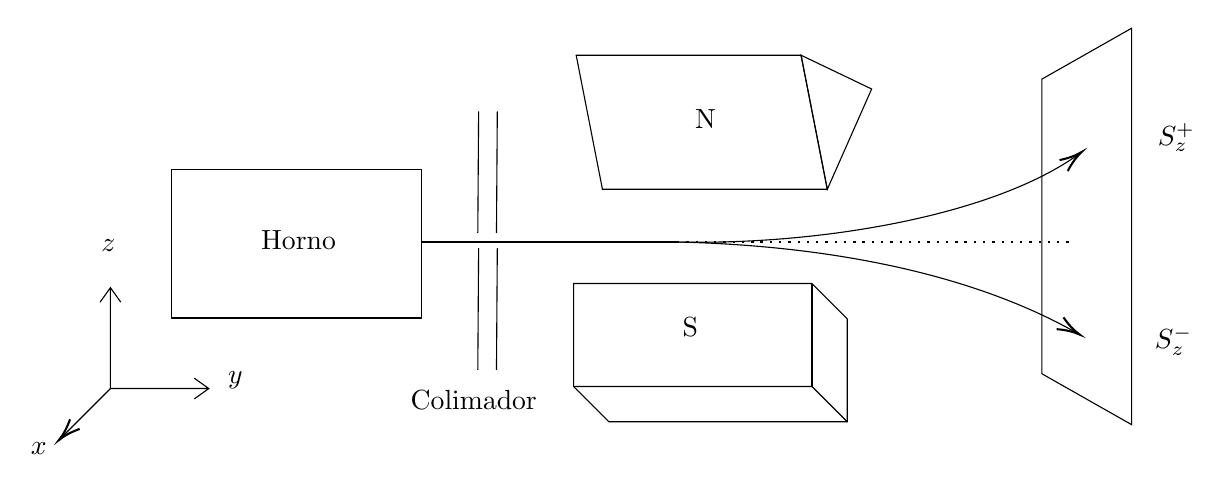
\begin{tikzpicture}[x=0.75pt,y=0.75pt,yscale=-1,xscale=1]
			%uncomment if require: \path (0,480); %set diagram left start at 0, and has height of 480

			%Shape: Cube [id:dp24345312390494178] 
			\draw   (329.74,256.6) -- (346.74,273.6) -- (461.6,273.6) -- (461.6,224) -- (444.6,207) -- (329.74,207) -- cycle ; \draw   (461.6,273.6) -- (444.6,256.6) -- (329.74,256.6) ; \draw   (444.6,256.6) -- (444.6,207) ;
			%Shape: Parallelogram [id:dp10384306412912792] 
			\draw   (343.66,161.6) -- (451.99,161.6) -- (439.34,97) -- (331,97) -- cycle ;
			%Shape: Triangle [id:dp17225841691105837] 
			\draw   (451.99,161.6) -- (473.35,113.28) -- (439.34,97) -- cycle ;
			%Shape: Rectangle [id:dp3058503225060799] 
			\draw   (136,152) -- (256.6,152) -- (256.6,223.6) -- (136,223.6) -- cycle ;
			%Straight Lines [id:da813570487414599] 
			\draw    (284,190) -- (283.6,248.6) ;
			%Straight Lines [id:da06069555327821807] 
			\draw    (293,190) -- (292.6,248.6) ;
			%Straight Lines [id:da25285245976762105] 
			\draw    (284,124) -- (283.6,182.6) ;
			%Straight Lines [id:da5021436349614967] 
			\draw    (293,124) -- (292.6,182.6) ;
			%Straight Lines [id:da08256115078382398] 
			\draw    (256,187) -- (379.6,187) ;
			%Curve Lines [id:da6928483836766991] 
			\draw    (379.6,187) .. controls (449.89,188.58) and (532.92,173.9) .. (573.39,144.5) ;
			\draw [shift={(574.6,143.6)}, rotate = 143.13] [color={rgb, 255:red, 0; green, 0; blue, 0 }  ][line width=0.75]    (10.93,-3.29) .. controls (6.95,-1.4) and (3.31,-0.3) .. (0,0) .. controls (3.31,0.3) and (6.95,1.4) .. (10.93,3.29)   ;
			%Curve Lines [id:da486748835919226] 
			\draw    (379.6,187) .. controls (449.89,188.58) and (520.18,201.34) .. (572.03,230.71) ;
			\draw [shift={(573.6,231.6)}, rotate = 209.98] [color={rgb, 255:red, 0; green, 0; blue, 0 }  ][line width=0.75]    (10.93,-3.29) .. controls (6.95,-1.4) and (3.31,-0.3) .. (0,0) .. controls (3.31,0.3) and (6.95,1.4) .. (10.93,3.29)   ;
			%Shape: Trapezoid [id:dp2851846359147088] 
			\draw   (598.6,274.99) -- (555.35,250.46) -- (555.35,108.53) -- (598.6,84) -- cycle ;
			%Straight Lines [id:da0002854667411364975] 
			\draw  [dash pattern={on 0.84pt off 2.51pt}]  (379.6,187) -- (569.6,187) ;
			%Shape: Axis 2D [id:dp59234031102005] 
			\draw  (106.6,257.6) -- (154,257.6)(106.6,209) -- (106.6,257.6) -- cycle (147,252.6) -- (154,257.6) -- (147,262.6) (101.6,216) -- (106.6,209) -- (111.6,216)  ;
			%Straight Lines [id:da2640816906561392] 
			\draw    (106.6,257.6) -- (83.15,281.05) ;
			\draw [shift={(81.74,282.46)}, rotate = 315] [color={rgb, 255:red, 0; green, 0; blue, 0 }  ][line width=0.75]    (10.93,-3.29) .. controls (6.95,-1.4) and (3.31,-0.3) .. (0,0) .. controls (3.31,0.3) and (6.95,1.4) .. (10.93,3.29)   ;


			% Text Node
			\draw (178,180) node [anchor=north west][inner sep=0.75pt]   [align=left] {Horno};
			% Text Node
			\draw (387,122) node [anchor=north west][inner sep=0.75pt]   [align=left] {N};
			% Text Node
			\draw (381,222) node [anchor=north west][inner sep=0.75pt]   [align=left] {S};
			% Text Node
			\draw (250,257) node [anchor=north west][inner sep=0.75pt]   [align=left] {Colimador};
			% Text Node
			\draw (67,282.4) node [anchor=north west][inner sep=0.75pt]    {$x$};
			% Text Node
			\draw (101,184.4) node [anchor=north west][inner sep=0.75pt]    {$z$};
			% Text Node
			\draw (162,248.4) node [anchor=north west][inner sep=0.75pt]    {$y$};
			% Text Node
			\draw (610,128.4) node [anchor=north west][inner sep=0.75pt]    {$S_{z}^{+}$};
			% Text Node
			\draw (608.6,226.4) node [anchor=north west][inner sep=0.75pt]    {$S_{z}^{-}$};

		\end{tikzpicture}

		}
		\caption{Esquema experimental de Stern-Gerlach. Átomos de plata son evaporados utilizando un horno y son disparados a través de un colimador a lo largo de un campo magnético no homogéneo, y colisionan en una pantalla}
		\label{fig:stern-gerlach}
	\end{figure}

\end{frame}

\begin{frame}
	\textbf{Experimentos sucesivos de Stern-Gerlach}\\
	\justifying Consideremos ahora un \textbf{segundo} experimento que direcciona el campo magnético a lo largo del eje $x$ colocado en sucesión al primer experimento en $z$, bloqueando con una pantalla $S_z^-$.\\
	\textbf{Hipótesis}: Los electrones están en las configuraciones $S_z^+$, $S_x^+$ o $S_z^+$, $S_x^-$.\\
	\justifying \textbf{Tercer experimento} sucesivo en la dirección $z$ (como el primero)
	\begin{itemize}
		\item Clásica: Se espera que solo haya electrones $S_z^-$
		\item Resultados: La pantalla muestra los mismos resutados que el experimento individual en $z$, electrones en estados $S_z^+$ y $S_z^-$
	\end{itemize}
	\textbf{Conclusión}: La medición del segundo experimento destruye la información del primer experimento.
\end{frame}

\begin{frame}[c]
	\frametitle{Kets y Bras}
	En notación de \textbf{Dirac}, los resultados del experimento anterior se pueden describir por Kets
	\begin{equation*}
		\ket{S_x; \pm} = \pm \frac{1}{\sqrt{2}}\ket{S_z; +} + \frac{1}{\sqrt{2}}\ket{S_z; -}\,.
	\end{equation*}
	Si se orienta el segundo experimento en $y$ se debe usar la misma base, por lo que se necesita de coeficientes complejos:
	\begin{equation*}
		\ket{S_y; \pm} = \frac{1}{\sqrt{2}}\ket{S_z; +} \pm \frac{i}{\sqrt{2}}\ket{S_z; -}\,.
	\end{equation*}
	A un estado cuántico en \textbf{estado} $\psi$ se le denota por $\vert \psi \rangle$, elemento de un espacio vectorial complejo de Hilbert.
\end{frame}

\begin{frame}[c]
	\frametitle{Operadores}
	\jusifying Función sobre un espacio de estados con contradominio en otro espacio de estados. Se representan por $\hat{A}$.\\
	\justifying \textbf{Observable:} Operador hermitiano que representa una cantidad medible por experimento, y tiene eigenvalores reales. \\
	\justifying Dos observables se dicen compatibles si conmutan, es decir $[\hat{A}, \hat{B}] = 0$ y el orden de las mediciones no afecta el resultado. Si el conmutador es distinto de cero se dicen no compatibles.
\end{frame}

\begin{frame}[c]
	\frametitle{Principio de incertidumbre}
	text
\end{frame}

\begin{frame}[c]
	\frametitle{Cambio de base}
	text
\end{frame}

\begin{frame}[c]
	\frametitle{Matriz de densidad}
	text
\end{frame}

\begin{frame}[c]
	\frametitle{Ecuación de Schödinger}
	text
\end{frame}

\begin{frame}[c]
	\frametitle{Evolución temporal}
	text
\end{frame}

\begin{frame}[c]
	\frametitle{Imagenes de la MC}
	text
\end{frame}

\begin{frame}[c]
	\frametitle{Oscilador armónico cuántico (OAC)}
	text
\end{frame}

\begin{frame}[c]
	\frametitle{Operadores escalera}
	text
\end{frame}

\begin{frame}[c]
	\frametitle{Estados número del OAC}
	text
\end{frame}

\begin{frame}[c]
	\frametitle{Operadores cuadratura}
	text
\end{frame}

\begin{frame}[c]
	\frametitle{Óptica cuántica}
	text
\end{frame}

\section{Cuantización campo EM}

\begin{frame}[c]
	\frametitle{Ecuaciones de Maxwell}
	text
\end{frame}

\begin{frame}[c]
	\frametitle{Ecuación de onda}
	text
\end{frame}

\begin{frame}[c]
	\frametitle{Solución a la ecuación de onda}
	Repasar teoría de EDP's, EDO's, solución particular y homogénea
\end{frame}

\begin{frame}[c]
	\frametitle{Condiciones de la función de onda}
	text
\end{frame}

\begin{frame}[c]
	\frametitle{Condiciones de la función de onda}
	text
\end{frame}

\begin{frame}[c]
	\frametitle{Soluciones a los campos}
	text
\end{frame}

\begin{frame}[c]
	\frametitle{Energía electromagnética}
	text
\end{frame}

\begin{frame}[c]
	\frametitle{Cuantización del campo}
	text
\end{frame}

\section{Compresión y desplazamiento}

\begin{frame}[c]
	\frametitle{Propiedades de los estados número}
	text
\end{frame}

\begin{frame}[c]
	\frametitle{Fasores}
	text
\end{frame}

\begin{frame}[c]
	\frametitle{Estados coherentes}
	text
\end{frame}

\begin{frame}[c]
	\frametitle{Propiedades de los estados coherentes}
	text
\end{frame}

\begin{frame}[c]
	\frametitle{Simetrías y grupos}
	text
\end{frame}

\begin{frame}[c]
	\frametitle{Grupos de Lie}
	text
\end{frame}

\begin{frame}[c]
	\frametitle{Álgebra de Lie}
	text
\end{frame}

\begin{frame}[c]
	\frametitle{Operador desplazamiento}
	text
\end{frame}

\begin{frame}[c]
	\frametitle{Propiedades del operador desplazamiento}
	text
\end{frame}

\begin{frame}[c]
	\frametitle{Operador compresión}
	text
\end{frame}

\begin{frame}[c]
	\frametitle{Estado comprimido ideal}
	text
\end{frame}

\section{Función de Wigner}

\begin{frame}[c]
	\frametitle{Teoría de función de Wigner}
	text
\end{frame}

\begin{frame}[c]
	\frametitle{Función de Wigner para estados coherentes}
	text
\end{frame}

\section{Amplificador paramétrico}

\begin{frame}[c]
	\frametitle{Óptica no lineal}
	text
\end{frame}

\begin{frame}[c]
	\frametitle{Parametric down conversion}
	text
\end{frame}

\begin{frame}[c]
	\frametitle{Amplificador paramétrico (AP)}
	text
\end{frame}

\begin{frame}[c]
	\frametitle{Diagonalización del AP}
	text
\end{frame}

\begin{frame}[c]
	\frametitle{Estado inicial}
	text
\end{frame}

\begin{frame}[c]
	\frametitle{Función de Wigner del campo}
	text
\end{frame}

\begin{frame}[c]
	\frametitle{Expresión paramétrica de la función de Wigner}
	text
\end{frame}

\begin{frame}[c]
	\frametitle{Resultados}
	text
\end{frame}

\begin{frame}[c]
	\frametitle{Conclusiones}
	text
\end{frame}

\begin{frame}[c]
	\centering ¡Gracias por su atención!
\end{frame}

\end{document}






